\section[Additions for retake]{Additions to webshop for assessment retake}
\begin{figure}[htbp]%[6]{r}{.4\textwidth}
\centering
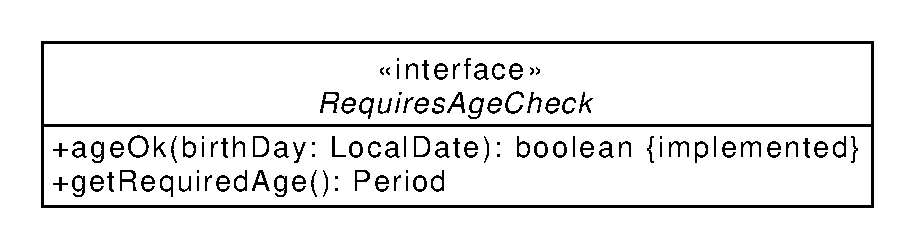
\includegraphics[width=.8\linewidth]{figures/booze.pdf}
\caption{\label{fig:booze}Product that requires age check.}
\end{figure}

The following additions have been made to the webshop in comparison to
the lab exercise:
\begin{description}
\item[java.time] API. In this new implementation the deprecated
  \sout{\Code{java.util.Time}} class and friends are avoided. Instead we use
  \Code{java.time.LocalDate} to represent Date values and \Code{ java.time.Period} to
  represent a time span, such as age.
\item[Age check] Product has a sub class called \Code{Booze} which
  requires an age check on sale. From the class diagram in
  figure~\ref{fig:booze} you can see the relation of the product
  subcategory \Code{Booze}, the \Code{Product} class and the new
  interface \Code{RequiresAgeCheck}.
\item[Persist invoice] On sale, the Invoice information is persisted in the database or
  in the in-memory persistence  implementation.
\item[File system persistence]
  the local  file system is used as a 'database', in which the entities, e.g. invoice, are
  persisted to one file each. In the invoice example, the whole
  invoice, including its lines, are persisted to said file.
  Each type has its own sub directory below the directory
  \texttt{./fsdb}.
  
  The mapper for the entities should be able to save the entity and
  restore the entity.

  To be able to implement this, you should use the \Code{java.io} or \Code{java.nio}
  API. HINT: look at \Code{ObjectOutputStream} and
  \Code{ObjectInputStream} classes Javadoc.
  
\end{description}
See the TODO list for the tasks these additions imply.


